\subsection{MFCC Quantization and Bounded Rice Compression}
\label{sec:mfcc_codec}
\newrevision{The packet-compaction design uses temporal delta encoding, zigzag mapping, and bounded Golomb--Rice coding. The supplied project codec notes describe a host benchmark and its reverse procedure. The receiving device in this project's updated architecture is an ESP32 cluster head. The same decoding procedure may run at the receiving endpoint or cloud, subject to implementation and resource testing. The notes' Raspberry Pi endpoint describes the earlier design.}

\begin{figure}[htbp]
\centering
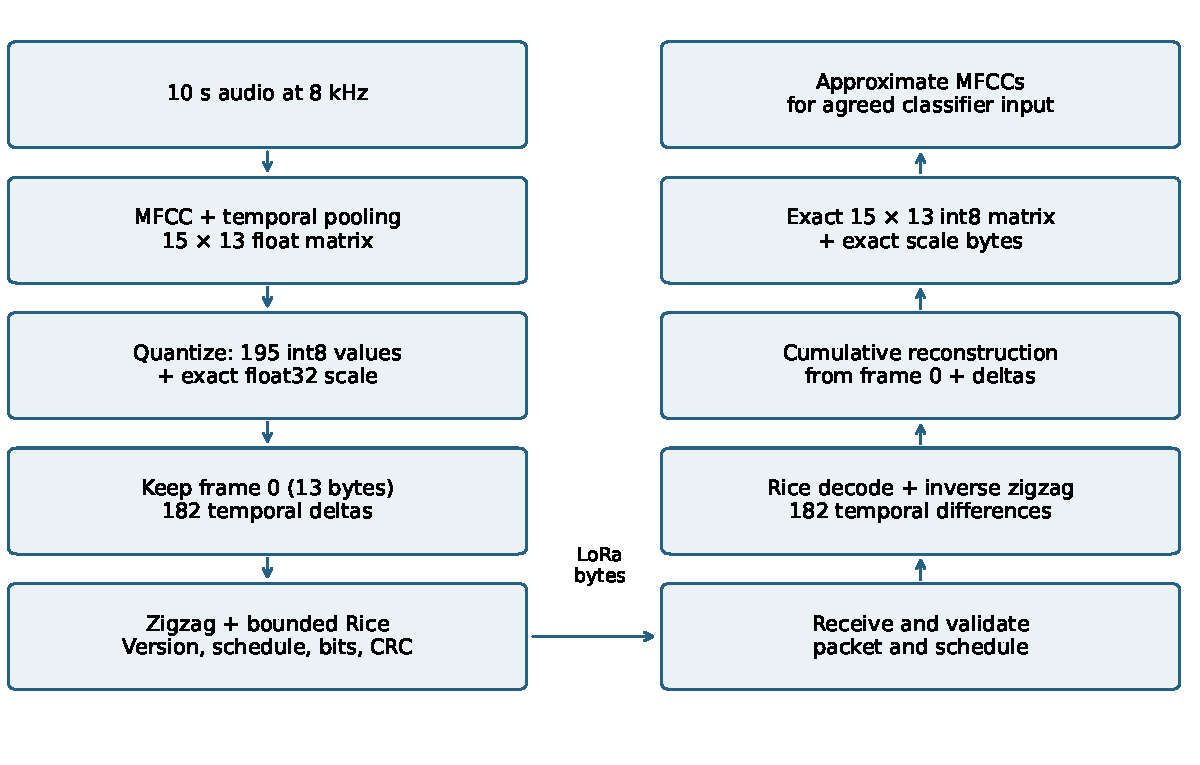
\includegraphics[width=\textwidth]{figures/mfcc_codec_pipeline.pdf}
\caption{\newrevision{MFCC encoding and reconstruction. The codec preserves the quantized matrix and scale exactly; audio and floating-point MFCC reconstruction remain lossy.}}
\label{fig:mfcc_codec}
\end{figure}

\begin{table}[htbp]
\centering
\caption{\newrevision{Reference MFCC extraction configuration supplied with the codec notes.}}
\label{tab:codec_frontend}
\begin{tabular}{p{0.28\textwidth}p{0.64\textwidth}}
\toprule
Stage & Configuration \\
\midrule
Input & Centre 10 seconds; stereo averaged to mono; shorter recordings excluded \\
Sampling & 8 kHz; 80,000 samples \\
Framing & 200-sample (25 ms) symmetric Hamming window; 80-sample (10 ms) hop; no end padding \\
Spectral transform & 256-point FFT power spectrum; 26 HTK-style mel filters over 0--4,000 Hz \\
Cepstral transform & Natural logarithm; orthonormal DCT-II; coefficients C0--C12 \\
Pooling & Average 998 complete frames in 15 consecutive groups; output $15\times13$ \\
Arithmetic & Float64 reference processing before quantization; one float32 scale \\
\bottomrule
\end{tabular}
\end{table}

\newrevision{The 15 output rows represent pooled time segments, rather than 15 original audio windows. This benchmark's 0--4,000 Hz mel configuration must be reconciled with the proposed 100--2,500 Hz node bandpass during frontend parity testing. Firmware and training must share windowing, pooling, normalization, rounding, and classifier input conventions. A codec round trip alone does not establish that parity.}

\newrevision{For floating-point matrix $M$, let $A=\max|M_{t,c}|$ and $s=\mathrm{float32}(A/127)$, using $s=1$ for an all-zero matrix. Quantization rounds $M_{t,c}/s$ to nearest even and clips to $[-127,127]$, producing 195 int8 values. The exact four scale bytes are retained. MFCC extraction, pooling, and quantization lose information relative to the recording; the subsequent codec is lossless relative to these integers and scale bytes. It cannot reconstruct the original WAV.}

\newrevision{The encoder stores all 13 values of the first pooled frame verbatim. For the remaining frames it computes $D_{t,c}=\mathrm{int16}(Q_{t,c})-\mathrm{int16}(Q_{t-1,c})$, yielding 182 temporal differences in time-major order. Subtraction uses at least 16-bit arithmetic to prevent overflow. For example, $[40,42,43,43,44]$ becomes an initial value of 40 and differences $[2,1,0,1]$; cumulative addition recovers the original sequence. Adjacent coefficients within a frame are never subtracted.}

\newrevision{Zigzag mapping converts each difference to $u=2d$ for $d\geq0$ and $u=-2d-1$ otherwise. With coefficient parameter $k_c\in\{0,\ldots,7\}$, the encoder computes $q=\lfloor u/2^{k_c}\rfloor$ and $r=u\bmod2^{k_c}$. If $q<15$, it writes $q$ one bits, a zero terminator, and exactly $k_c$ remainder bits. Otherwise it writes 15 one bits followed by the 9-bit literal $u$, without a terminator or remainder. This bounds a delta code at 24 bits. The generic int8 difference range is $[-255,255]$; the specified quantizer's $[-127,127]$ outputs give the narrower $[-254,254]$ range. Both fit the escape representation.}

\newrevision{For $k=0$, differences $[0,-1,+1,+2]$ encode as $0\,|\,10\,|\,110\,|\,11110$. Concatenating and padding these 11 meaningful bits gives bytes \texttt{0x5B 0xC0} in most-significant-bit-first order. The decoder uses the meaningful bit count and expected symbol count to distinguish information from zero padding.}

\begin{table}[htbp]
\centering
\caption{\newrevision{Rice schedule alternatives and experimental packet overhead.}}
\begin{tabular}{p{0.21\textwidth}p{0.39\textwidth}p{0.31\textwidth}}
\toprule
Method & Schedule choice & Decoder information \\
\midrule
Fixed & One trained 13-parameter vector & Matching provisioned version \\
Per packet & Best parameter for each coefficient in this recording & 39 descriptor bits, padded to 5 bytes \\
Predefined bank & Small trained bank; select the shortest candidate & Versioned registry and selector; benchmark charged selector within header flags \\
\bottomrule
\end{tabular}
\end{table}

\newrevision{A coefficient's parameter applies to its 14 differences throughout a packet. This is schedule selection, rather than parameter adaptation after every symbol. The experimental raw reference is 209 bytes: 195 feature bytes plus a 14-byte envelope that already includes the four-byte scale. Compressed packets contain that envelope, the 13-byte first frame, any schedule descriptor, and the byte-padded delta stream. A raw fallback is available when compression is larger. Final node ID, timestamp, application headers, and radio framing must be budgeted separately unless the chosen protocol explicitly includes them. The older example envelope offsets in the notes are not a verified specification of the newer benchmark. Firmware interoperability still requires its actual wire-format definition, schedule registry, and golden vectors.}

\newrevision{The receiver validates the mode, length, version, integrity check, finite positive scale, schedule identity, meaningful bit count, and padding. It reconstructs exactly 182 symbols using $c=i\bmod13$, reverses zigzag, and adds each difference to the same coefficient in the previous time frame. It rejects truncated codes, invalid escapes, out-of-range reconstructed values, and unexpected remaining bits. The result is the original quantized $15\times13$ matrix and exact scale bits. Optional dequantization gives $\widehat M=sQ$ under the classifier's agreed arithmetic.}

\subsubsection{Reported Host Compression Benchmark}
\newrevision{The supplied notes report the complete experimental packet sizes in Table~\ref{tab:codec_results}. Raw benchmark records and sample counts were not supplied with the explanation, so these values are reported project results awaiting reproduction. They provide no classification, measured radio airtime, or ESP32 runtime evidence.}

\begin{table}[htbp]
\centering
\caption{\newrevision{Reported held-out packet sizes for the validation-selected schedule bank.}}
\label{tab:codec_results}
\begin{tabular}{lrrr}
\toprule
Dataset & Mean bytes & p99 bytes & Mean reduction vs. 209 bytes \\
\midrule
LAB & 59.68 & 65 & 71.4\% \\
FIELD & 80.40 & 103 & 61.5\% \\
FARM-LIKE proxy & 72.16 & 98 & 65.5\% \\
\bottomrule
\end{tabular}
\end{table}

\begin{figure}[htbp]
\centering
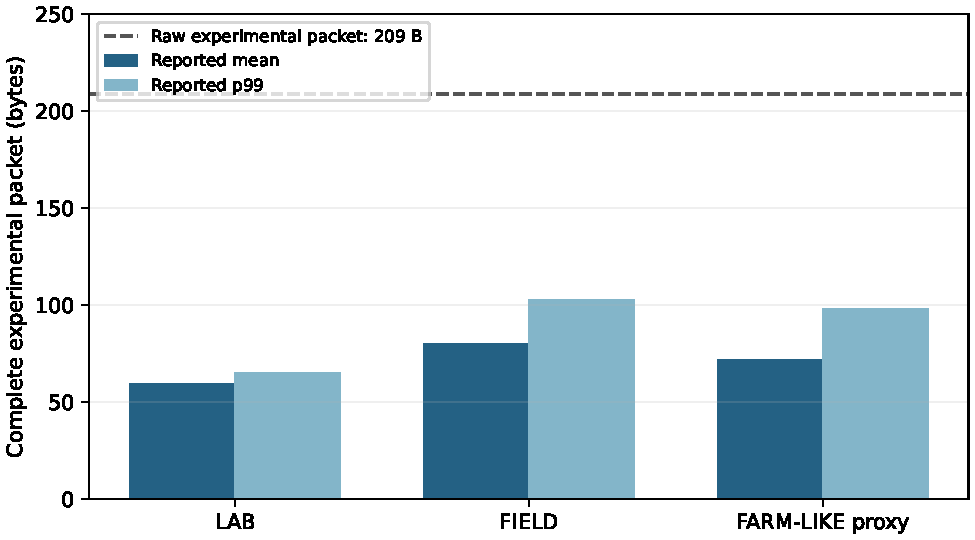
\includegraphics[width=0.93\textwidth]{figures/mfcc_packet_comparison.pdf}
\caption{\newrevision{Reported experimental packet sizes. Each dataset used a different trained schedule model. The FARM-LIKE proxy overlaps FIELD and is not confirmed date-palm-farm data.}}
\label{fig:codec_sizes}
\end{figure}
\newrevision{Verification will include byte-for-byte round trips of zero, alternating-sign, extreme-int8, and random matrices, followed by shared golden packet vectors. Payload reduction will be evaluated separately from packet delivery, energy, frontend parity, and detection performance.}
\FloatBarrier
